\subsection{Level3.2: パラメータと収束能力の関連性について}
\subsubsection{関係性を確認するためのアプローチ}
文字認識プログラムnn\_numではいくつかのパラメーターが設定されているが,今回はETA,ALPHA,HIDDENに着目する.
これらパラメーターが収縮能力にどのような影響を及ぼすのかを今回は考察する.
尚,起動時にはもう1つパラメーターとしてseed値を入力する必要がある.
しかし今回のプログラムではseedはあまり関係が無く学習が収束する.
従って今回の検証ではseed値は1000に固定を行った.

\subsubsection{実際の検証について}
今回実際に検証するに対して,前述の3種類のパラメーターの影響を考察する.
方法としては確認対象のパラメーターを変動させ,それ以外のパラメーターを固定した状態で実際に学習を行う.
この出力結果を比較し,それぞれがどの様な影響を及ぼすかを調査した.
Level3.1では幾つかのパターンで総当りを行ったが,今回の実験では実際にこれら全てのデータは使用しない.
それぞれのパラメーターに対して,実行した数値から3つ選び,実行した.
実行結果から比較を行い,今回は合計9回学習を行っている.

探索では幾つかのシェルスクリプト.及びグラフのplotにgnuplotを用いた.

今回検証したパターンを示す.


\begin{itemize}
    \item ALPHA 0.50 HIDDEN 5に設定
        \begin{itemize}
        \item ETA 0.01 の場合
        \item ETA 1.00 の場合
        \item ETA 1.98 の場合
        \end{itemize}
    \item ETA 1.50 HIDDEN 5に設定
        \begin{itemize}
            \item ALPHA 0.01 の場合
            \item ALPHA 1.00 の場合
            \item ALPHA 1.98 の場合
        \end{itemize}
    \item ALPHA 0.50 ETA 1.0に設定
        \begin{itemize}
            \item HIDDEN 1 の場合
            \item HIDDEN 5 の場合
            \item HIDDEN 15 の場合
        \end{itemize}

\end{itemize}

今回収縮能力を考察するにあたり,run\_nn.bashを一部改良し利用した. 変更部分をdiffコマンドを用いて表す. (ソースコード:\ref{nnbashr})
\lstinputlisting[caption=run\_nn.bashの変更点,label=nnbashr]{nnbash.diff}
主な変更点は,タイトルの表示を今回変更したパラメーターに対応させ,seed値を1000で固定した.
また\LaTeX でレポートを作成する際にPDF形式が編集し易い為,出力形式をpdfに変更した.

今回はこのスクリプトと,nn\_num内で実行する処理を記述したcommand2.txtを用いて動作させた.
以下に今回実行したコマンド例を示す.
\begin{oframed}\begin{verbatim}
$bash nn_num "HIDDEN5" < command2.txt
      \end{verbatim}
\end{oframed}

尚パラメーターの変更は,自動化するべきであったが,手動でヘッダーファイルを編集し都度makeを実行した.

\subsubsection{結果}

まずETAを変更した場合の実行結果を示す. (図:\ref{fig:ETAresult})
処理の段階で,先程のbashスクリプトで一つずつのグラフを作成している.
しかし,今回はパラメーターを変更した場合の比較を確認したい為,各条件で処理を実行した後に纏めてグラフ化を行った.
グラフ化にはシェルスクリプトを用いたが,各処理はおおよそ共通している.
その為,今回レポートで示すシェルスクリプトは一つとする. (ソースコード:\ref{gnuplotALPHA})

\lstinputlisting[caption=gnuplotALPHA.sh,label=gnuplotALPHA]{../nn/nn_num/src/gnuplotALPHA.sh}

今回はplotしたいテキストファイル名が既に確定していた為,静的にスクリプト内に記述している.
もし大規模な実験データをplotする場合,ある一定の命名規則に則ったテキストファイルをplotするような記述に
変更するべきであると考える.
また,gnuplotでpdf出力を選択した場合replotを繰り返すと同一pdfファイル内にreplotした時点での画像データが
新しいページとして保存される.
今回はまとめたデータのみ必要だった為,全てreplotした後に出力先をpdfに変更しreplotしている.

\begin{figure}[H]
    \centering
    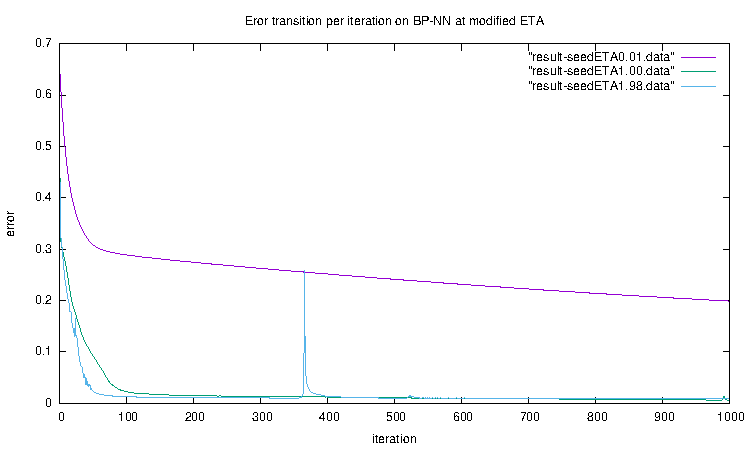
\includegraphics[width=0.8\textwidth]{figs/Level3.2/ETA.pdf}
    \caption{ETAの値を変更した場合の推移}
\label{fig:ETAresult}
\end{figure}

グラフを確認すると,ETAの値が大きくなるに連れてerrorの数値が減少している事が読み取れる.
また,共通して初回のerrorが大きく,iterationの回数が増えていくにつれてerrorが減少していく.
ETA1.98の場合,300から400の間で一度極端にerrorの値が上昇しているが,これは必ずしもerrorが改善されないことに起因していると推測する.
この実家から,ETAに関してはなるべく大きな数値で実行するとerrorの発生を抑えられることが判断出来る.

続いてALPHAの値を変更した場合の挙動を確認する. (図:\ref{fig:ALPHAresult})

\begin{figure}[H]
    \centering
    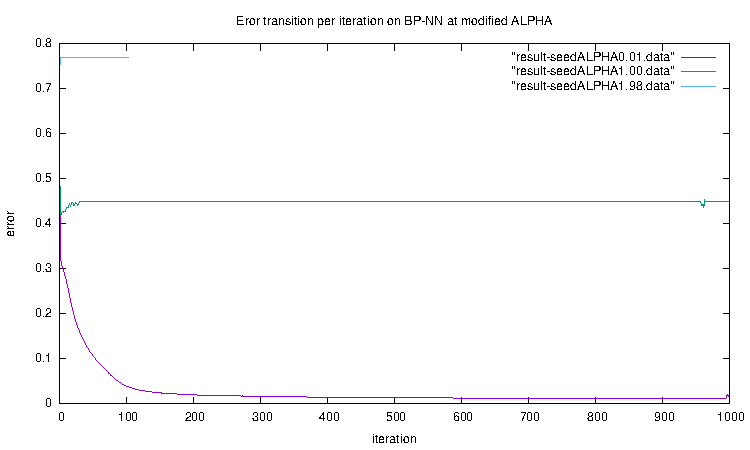
\includegraphics[width=0.8\textwidth]{figs/Level3.2/ALPHA.pdf}
    \caption{ALPHAの値を変更した場合の推移}
\label{fig:ALPHAresult}
\end{figure}

この図を確認すると,ALPHAの値が0.01の場合,errorがiterationを重ねるに連れて減少していくことが読み取れる.
しかし,ALPHAの値を1.0にした場合は,むしろ初回よりerrorが上昇した.
さらにiteration 100以降の場合はほとんどerrorの値に変化が見られなかった.
1.98の場合はiteration100を超えた場合,正常にerrorの結果がプログラムから取得出来なかった.
従って,慣性項ALPHAに関しては今回の結果から考察すると0に近い数値にするとより良く収束する.
また,数値を大きく取ってしまうと,正常に実験が出来ないと推測する.

最後にHIDDENの値を変化させた場合の挙動を確認する. (図:\ref{fig:HIDDENresult})

\begin{figure}[H]
    \centering
    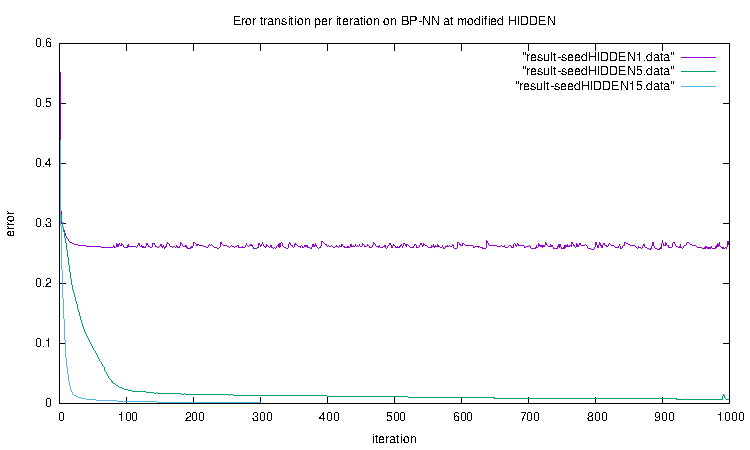
\includegraphics[width=0.8\textwidth]{figs/Level3.2/HIDDEN.pdf}
    \caption{HIDDENの値を変更した場合の推移}
\label{fig:HIDDENresult}
\end{figure}

実行結果からHIDDENの値を1にした場合,微少に上限に変動し続けるが,おおよそerrorが一定の値を保つ事がわかる.
しかし,5,15にHIDDENの値を設定した場合,iteration 100までで急激にerrorが低下し,以降は一定という挙動を示した.
さらにHIDDENを15にした場合,他の2種類よりiterationの回数が圧倒的に低かった.

\subsubsection{考察}
今回の実行結果を確認するとETAの値は1.98,ALPHAが0.01,HIDDENが15の場合それぞれ良い収束結果を見せた.
中間層ユニットHIDDENの数は学習結果を集約させしすぎてしまうと捨てられるデータが大きくなると推測する.
しかし,ある一定サイズより多く確保しても入力データそのものに対して違いが無い為,最終的なerrorの値は同様になると考える.

学習係数ETAは最急降下法と同じく探索点を更新する際の動きを制御するパラメーターである.
この値は小さい場合精度が上がると考えられるが,今回の場合iterationの収束を考えると1以上の大きさの値にするべきであると考察する.

慣性項は今回の場合,極力小さな値で実行するべきであると考える.
慣性の通り,前回の探索点との変化を示す\cite{sizuoka} 為,大きすぎると探索点の移動に支障が出てしまうと考える.
特に1.00にした場合ほとんど動かなかった.
以上のことよりこれらパラメーターを最適値にする場合,ある程度職人技のような微調整が必要であると考える.
